\chapter{History}\label{chap:history}

\begin{figure}[h!]
\begin{centering}
  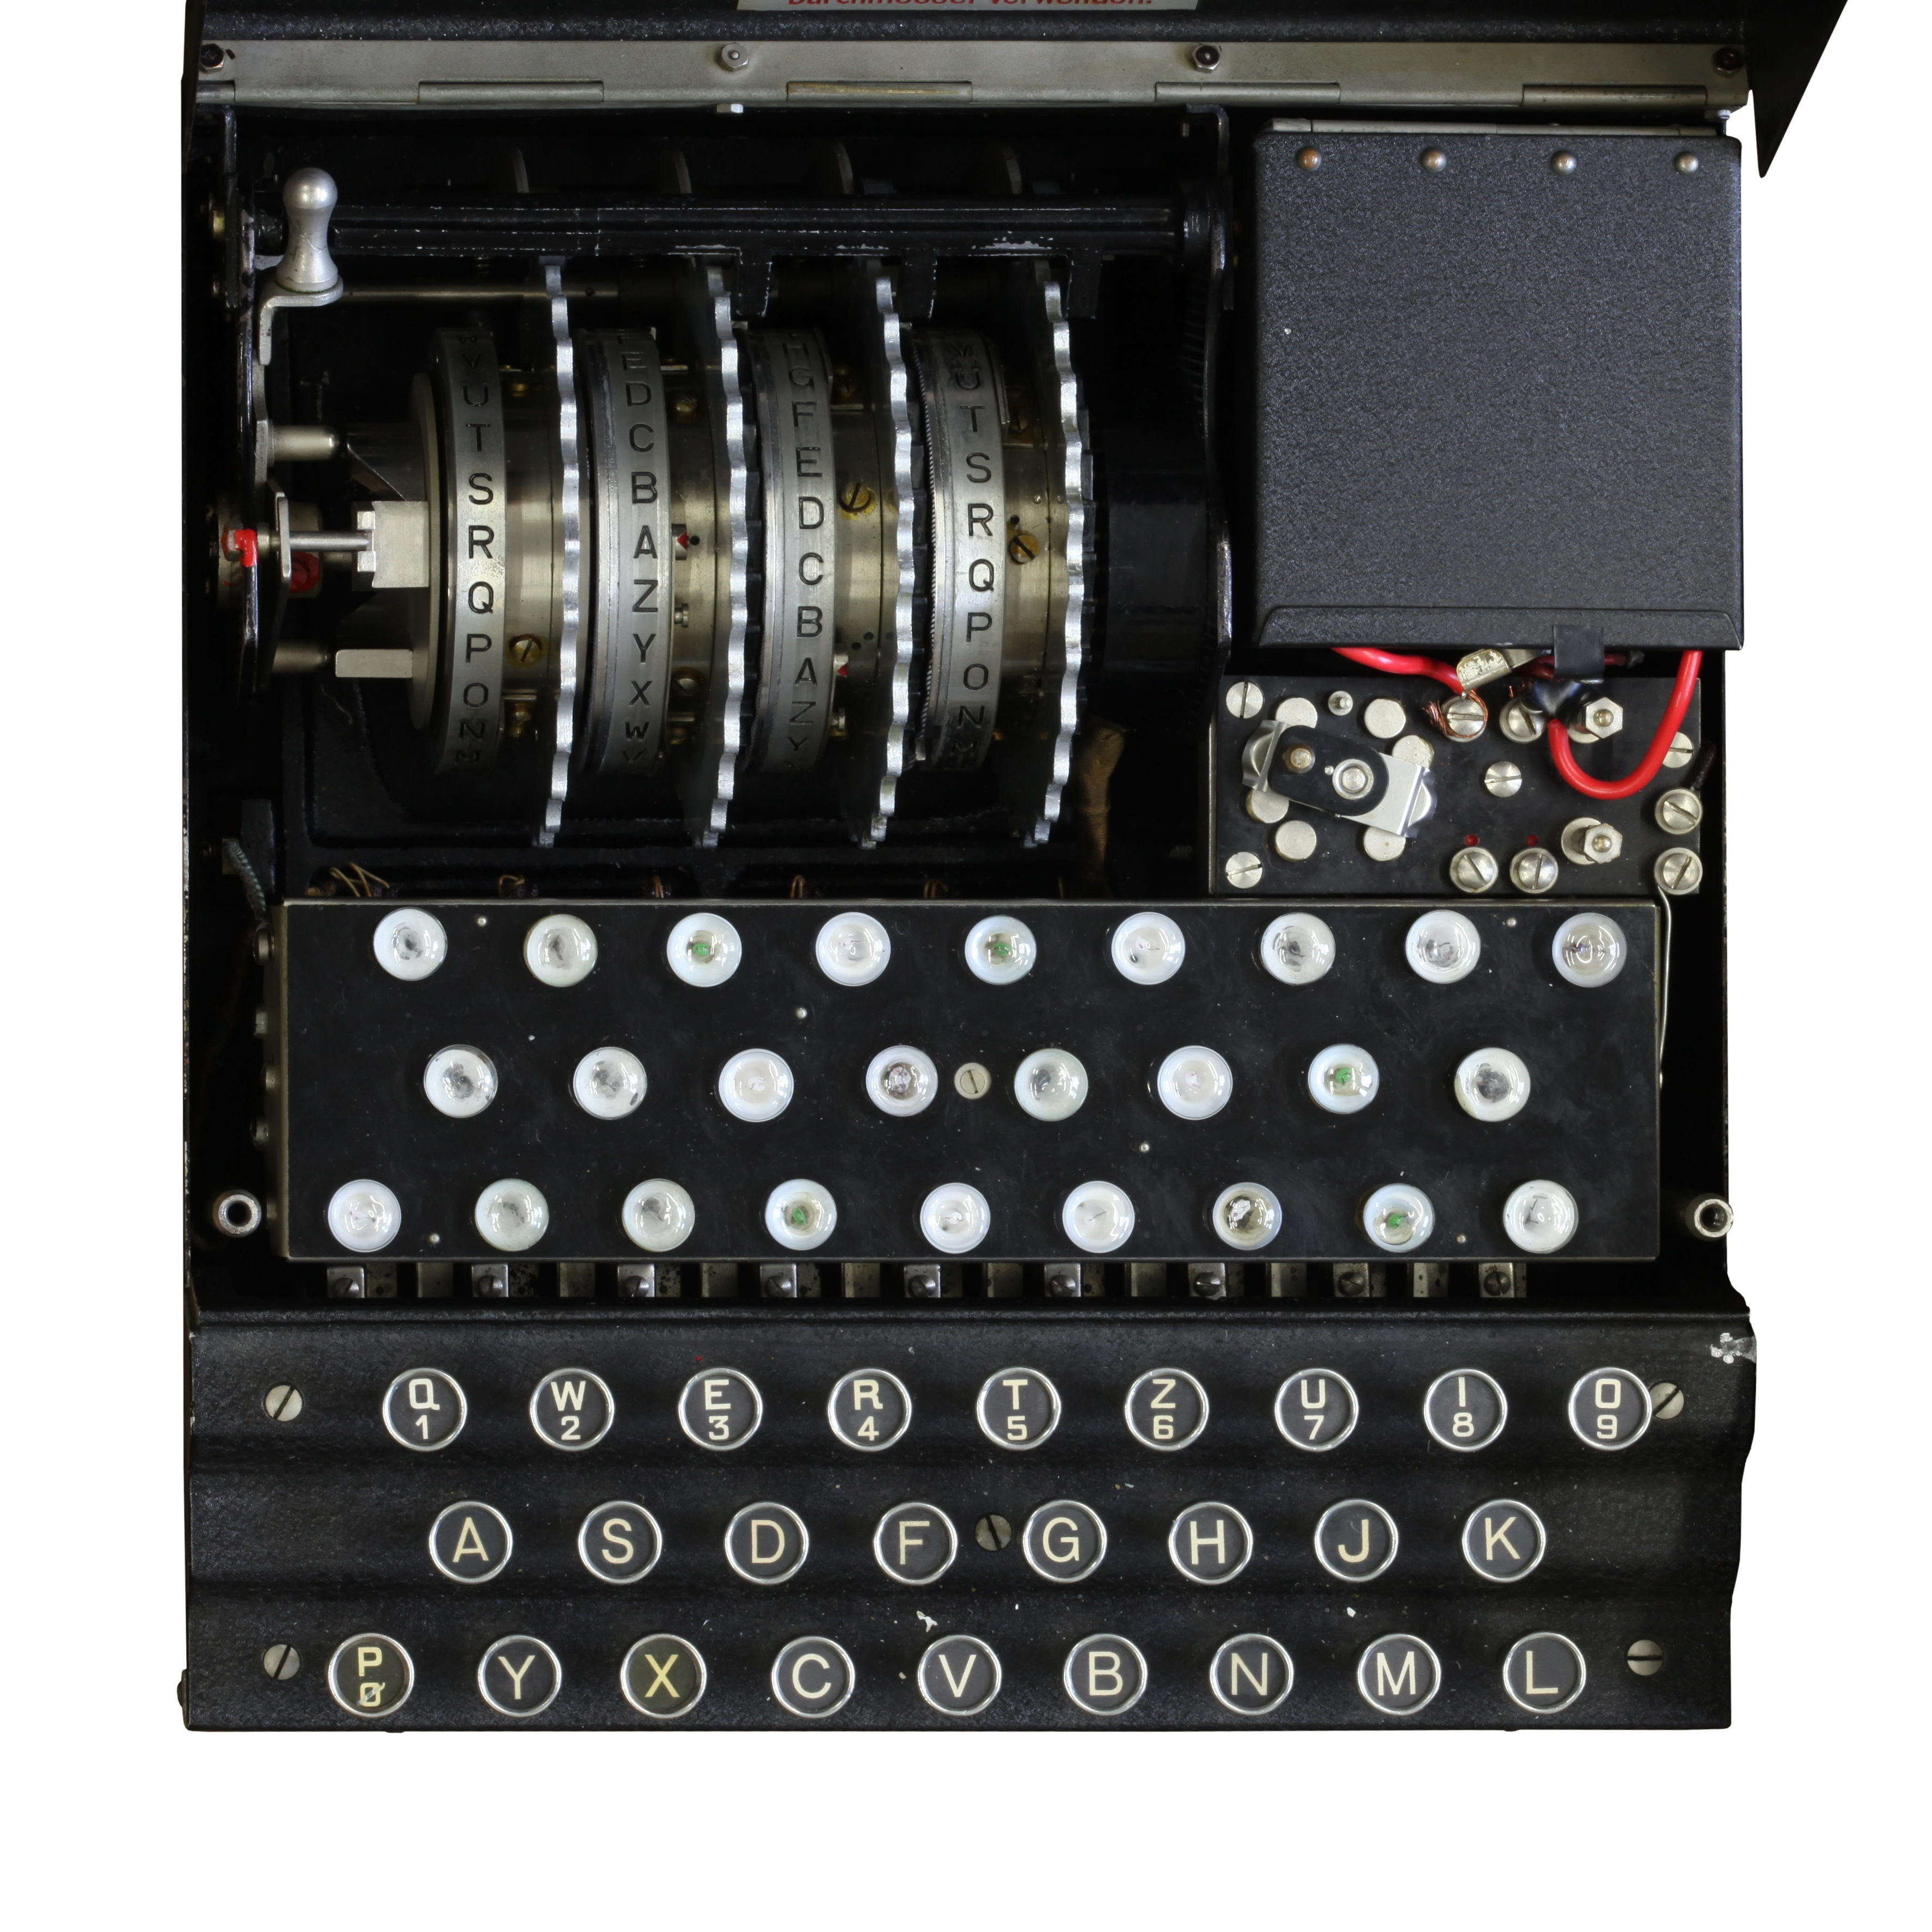
\includegraphics[height=6cm]{images/enigma.jpg}
  \caption{The Enigma Machine}
  \label{fig:machine1}
\end{centering}
\end{figure}

\section{Machine Encipherment}
In the First World War, war radios began to have an increasingly large role in military communications. The greatest advantage was the increased range of distance from which one could communicate, but the greatest disadvantage was that messages were easily intercepted. This led to cipher systems being developed, but because cipher clerks were not cryptanalysts or mathematicians, it was important to lmiit the complexity of these systems. If the system used to encipher a message was too complex, there was an increasingly high risk of error in the message, which could have had disastrous consequences in wartime. After the war, it was decided, in multiple countries, that the best way to encipher the messages was to have a user-friendly machine that would increase the complexity of encipherment, while decreasing the complexity of the tasks done by the cipher clerk. In the early 1920’s a German man, Arthur Sherbius, developed Enigma for this very purpose. Enigma was an iteration on several difference cipher machines that centered around using a large number of substitution alphabets, where no single alphabet would repeat until thousands of letters had been processed. The first Enigma was based on several main components: a twenty-six (26) letter keyboard, twenty-six (26) lamps to illuminate the ciphertext, a power supply, three (30) removable wired wheels that rotate on a common axis, a fixed wired reflector, and a fixed wired entry wheel \cite{rfc01}. Future iterations of Enigma would include a plug board where one could essentially swap two characters.

\section{Before the War}

The first Enigma was shown in 1923 at the Universal Post Union Congress in Vienna. Soon after, Germany began to adopt the machines for military and government communications and used them without much issue for many years. It wasn’t until 1930, with tensions remaining at a high level in Europe, that Poland felt the need to start protecting themselves from Germany by arming themselves with knowledge. They began intercepting German messages to attempt to decipher them. In the early 1930s, Captain Gustave Bertrand, a member of the French General Staff, took initiative to communicate with his opposite but equal peer in the Polish General Staff, after the French General Staff rejected a proposal by Poland to coordinate their intelligence gathering. Thanks to the direct communication between the men of different nations, intelligence gathered by France, particularly that which related to solving Enigma, was discreetly shared with Poland; not the least of which was operating instructions and keying instructions of Enigma. The operating instructions helped the Polish Cipher Bureau determine the inner workings of the military Enigma machines. The keying instructions, outlined in \secref{sec:encprocess1938}, helped the cryptanalysts understand how the messages they were intercepting were structured. In early 1933 the Polish Cipher Bureau team had deduced the inner workings of Enigma and has commissioned the building of fifteen duplicates. Duplicating the machine, however, was not enough since the machines also had to be given the correct settings to decipher a message correctly. These settings were the public key that had to be transmitted with cipher text. At first they were simply found by process of elimination. In 1934 a member of the Polish Cipher Bureau team, Marian Rejewski, created the cyclometer, which allowed the team to create a catalog of characteristics (possible permutations of the rotor closest to the keyboard) from the over 100,000 possible settings \cite{rfc01}. This made it much easier to find a key based on a given ciphertext, because a cryptanalyst could compare it with the catalogued characteristics. The cyclometer, along with several other tools and practices, enabled the team to successfully and consistently decipher messages for over 5 years.

\section{Enigma in World War II}

In 1938, Germany made an effort to increase the complexity and security of their system by changing the keying practices, allowing for rotors to be placed in various slots and other small changes to their enciphering practices. At the same time, the Polish Cipher Bureau team was making strides toward further automating the discovery of message keys. The Cryptological Bomb, or Bomba, was an electromechanical machine that would iterate over 17,000 possibilities in under 2 hours, stopping automatically when the desired one was found, and would turn on an indicator light. Also around this time, Germany began to occupy its neighboring nations, beginning with Austria. Throwing European politics into chaos, Britain and France were both looking for an ally with which to align themselves. Poland arose as the choice, and shortly before Germany’s occupation of Poland in late 1939, there was a meeting of the three nations where Poland’s accomplishments were shared, along with a great number of documents and resources, including one of the duplicate Enigma machines. As soon as the German forces made way into Poland, all work and remnants of the work done by the Cipher Bureau was destroyed, as the team of cryptanalysts fled to France. Before the end of the year, Britain had established Bletchley Park, the campus where the Ultra team would work to continue what the Polish Cipher Bureau had started. By all definitions, the Polish broke Enigma, and the British capitalized on their given knowledge to find solutions in record time \cite{rfc01}. They were both extremely important to wartime intelligence. The British Bomb, or Bombe, was developed by Alan Turing, who began work on the machine just after Britain’s first meeting with Poland and France. It accomplished the same task of the Bomba, to determine the keyspace for a given ciphertext, but the Bombe looked at the entire text rather than just the encrypted settings at the beginning of the message. This enabled the machine to find a solution in 20 minutes rather than 2 hours. The accomplishments of each nation held great significance in the war and the efforts towards bringing it to an end.
